% This is samplepaper.tex, a sample chapter demonstrating the
% LLNCS macro package for Springer Computer Science proceedings;
% Version 2.20 of 2017/10/04
%
\documentclass[runningheads]{llncs}
%<
\renewcommand\labelitemi{$\bullet$}
\usepackage{graphicx}
% Used for displaying a sample figure. If possible, figure files should
% be included in EPS format.
%
% If you use the hyperref package, please uncomment the following line
% to display URLs in blue roman font according to Springer's eBook style:
% \renewcommand\UrlFont{\color{blue}\rmfamily}

\begin{document}
%
\title{Cloud Computing Systems Work Report}
%
%\titlerunning{Abbreviated paper title}
% If the paper title is too long for the running head, you can set
% an abbreviated paper title here
%
\author{Bruno Cabrita\inst{57833} \and
Diogo Almeida\inst{58369} \and
Diogo Fona\inst{57940}}
%
\authorrunning{B. Cabrita, D. Almeida, D. Fona}
% First names are abbreviated in the running head.
% If there are more than two authors, 'et al.' is used.
%
\institute{NOVA School of Science and Technology - MSc in Computer Engineering 
\email{\{brm.cabrita,daro.almeida,d.fona\}@campus.fct.unl.pt}}
%
\maketitle % typeset the header of the contribution
%
%
\section{Introduction}
%briefly explain the context and goal of the system being developed
The goal of this work is to understand how services available in cloud computing platforms can be used for creating applications that are scalable fast, and highly available.

\subsection{Context}
This work consists in the design and implementation of the backend for an auction system like E-Bay and companion scripts for testing the system.

The system will manage auctions. Users can create auctions and bid on open auctions. A user can also pose questions about the product of an auction. A question can only be answered by the user that created the auction, and there can be only one answer for each question.


\section{Design}

In this section we briefly discuss the system's design, explaining what information it holds, what components it uses, and endpoints for client communication.

\subsection{Architecture}

The system mantains the following information:
\begin{itemize}
    \item \textbf{Users}: information about users, including the nickname, name, (hash of the) password, photo;
    \item \textbf{Media}: manages images and videos used in the system;
    \item \textbf{Auctions}: information about auctions, including for each auction a title, a description, an image, the owner (the user that created the auction), the end time of the auction (i.e. until when bid can be made), the minimum price, the winner bid for auctions that have been closed, the status of the auction (open, closed, deleted).
    \item \textbf{Bids}: Each bid includes the auction it belongs to, the user that made the bid and the value of the bid.
    \item \textbf{Questions}: auctions' questions and replies. Each question includes the auction it refers to, the user that posed the question and the text of the message. 
\end{itemize}

To support the storage, querying, and processing of this information, we use the following cloud software and hardware components. In our work these are provided by Microsoft Azure.

\begin{description}
    \item[App Service] which clients interact directly with. Afterwards the service communicates with other components to return information to the clients. The software running in this service is implemented by us in Java.
    \item[Database] that stores the information of the objects described above in a structured way and allows querying them. In this work we use CosmosDB as the database.
    \item[Blob Storage] that stores binary data, images and videos of users and auctions in this context.
    \item[Cache] which stores query and computation results, so later requests of the same information doesn't need to be queried or computed again. In this work we use Redis for caching.
    \item[Serverless Functions] that do additional computations that don't need to be constantly running in the App Service. We use Azure Functions to provide this service.
    \item[Message Queues] on which the app service sends events to, as the publisher, and some app functions are subscribed to, to support some functionality. These are implemented with Azure's Service Bus Namespace.
    \item[Search Service] which provides search approaches based on AI, like searching for relevant information based on a text query. We use Azure Cognitive Search for the searching service.
\end{description}

Some of these components (App Service, Database, Blob Storage and Cache) can have multiple replicas/instances.

\subsection{Endpoints}

The App Service provides the following REST endpoints for communication with clients. The descriptions encompass a number of endpoints, having the following as the base ones:

\begin{itemize}
    \item \textbf{Users} (/rest/user): Create, authenticate, get, delete and update a user. List auctions a user has created and has bidded for;
    \item \textbf{Media} (/rest/media): Upload and download media;
    \item \textbf{Auctions} (/rest/auction): Create, get and update an auction. List auctions that were recently created, are closing soon, and popular ones. Query auctions.
    \item \textbf{Bids} (/rest/auction/\{id\}/bid): Bid for an auction or list its bids;
    \item \textbf{Questions} (/rest/auction/\{id\}/question): Post a question on an auction, reply to a question and list an auction's questions. Query questions from an auction.
\end{itemize}


\section{Implementation}

In this section we provide some details on some relevant aspects of the implementation in regards to the topic of cloud computing systems.

\subsection{Database Operations}

The "delete" operations, deleteUser and closeAuction, are set to strong consistency level, as we want to assure that unwanted operations are not requested on these objects, such as a deleted user being read or a closed auction gettings bids.

The remainder of operations are set to session consistency level to assure that a client reads his writes and mantain good availability.

To handle concurrent bids for an auction, we implemented a conditional update where an auction's winning bid is only updated when the previously read one has the same id and the auction is open. If this fails, it retries the operation until it completes or until the auction closes.

Important to note that in our implementation a user isn't truly deleted but "soft deleted", in the same way auctions are updated to "closed". This way, all references to the id of a deleted user are shown as "deleted".

\subsection{Caching}

We store in Redis cache all objects (User, Auction, Bid and Question DAOs) until they are invalidated by either timeout, after 1 hour (or another configurable value), or are updated, in which they must be replaced in the cache, or deleted. 

Lists of IDs of these objects are formed in cache with each write operation. These constitute the result of some operations such as listing 1. a user's auctions, 2. a user's followed auctions, 3. an auction's bids and 4. an auction's questions, and also for saving the winning bid of each auction. The objects can then be retrieved using their IDs from cache. 

The advantage of this approach is when an object is updated, since the lists are of immutable IDs we don't need to invalidate one which contained that object. 

The disadvantage of this is we need to get each of the objects through their IDs from the cache, or database in the worst case. To amortize this (this isn't currently implemented), we could bundle all IDs and get their respective objects in one request.

Additionally we keep track of results of some listing operations which involve ordering. This is possible with Redis's sorted sets and incrementing scores. Those operations are the listing of the closing auctions (ordered by the closest auction's end time), of the recent auctions (ordered in list on insertion), and of popular auctions (ordered by number of bids on them, which are incremented with every added bid). The top 20 of each operation are returned to the application.

The listing of recent and popular auctions in particular need to have cache enabled to work, meaning these queries are not computed in the database.


\subsubsection{Session Keeping}

Using Redis cache, we keep the session keys of users after they authenticate in the system. Each session key expires in 30 minutes, after which users need to authenticate again to use the system. Furthermore some subsystems could be implemented over this: the session key could be removed after the user "logs out"; after each operation the expire time is refreshed (idle logout system).

\subsection{Serverless Functions}

We implemented some serverless functionality, using Azure Functions,  that perform some periodic computations as described: 

\subsubsection{Auctions about to Close}

Every 2 minutes, queries the database looking for the auctions that are about to close and fills the Redis cache with that information. The application then requests Redis for these auctions when there's a client request as mentioned before.

\subsubsection{Closed Auctions}

When an auction is created, the application sends an event to a message queue scheduled to deliver on the time the auction is closing. This function is subscribed to that message queue and when it receives the message corresponding to an auction (only on the moment that the auction should close due to the schedule) it requests the databe to set the auction's state to closed.

\subsubsection{Popular Auctions}

This functionality is divided in two functions with two separate behaviours:
\begin{enumerate}
    \item Whenever a bid is inserted in the database, it increments the amount of bids made to that auction in Redis;
    \item Every 2 minutes, removes from cache the 20 auctions with the highest amount of bids. This meaning the notion of popularity in our system is temporary.
\end{enumerate}

\subsubsection{Recent Auctions}

This function is triggered whenever one or more auctions are created in the database. These auctions are inserted in cache where the size of the list is limited to 20. The application afterwards requests Redis for this list of most recent auctions.

\subsubsection{Delete User}

When a client requests to delete a user the application sends an event to a message queue. This function is subscribed to that message queue and when it receives the messages corresponding to a user it queries the database to delete its object. This way, the operation is asynchronous in the point of view of the user.

\subsubsection{Blob Replication}

To implement blob replication through data centers in different regions, which is not a feature provided by Azure in our Student Plan, we use a function that triggers when media is uploaded to a blob in one data center and uploads it to the other blobs in other data centers (in our case one other). Note that in this way the replication is asynchronous.

\subsection{Advanced Search}

Using Azure Cognitive Search we implement operations that do queries based on text, where relevant results, not necessarily exact text matches, are returned. The operations in question retrieve auctions, and questions of an auction, based on a text search.

\section{Evaluation}

In this section we evaluate our work, and demonstrate why the use of technics such as caching and geo-replication are opportune.

The evaluation was done running workload tests with Artillery from a single client located in Lisbon, Portugal. For tests with geo-replication, we execute two clients, in the same location, each communicating with a different replica (West Europe or Central US).

\begin{figure}
    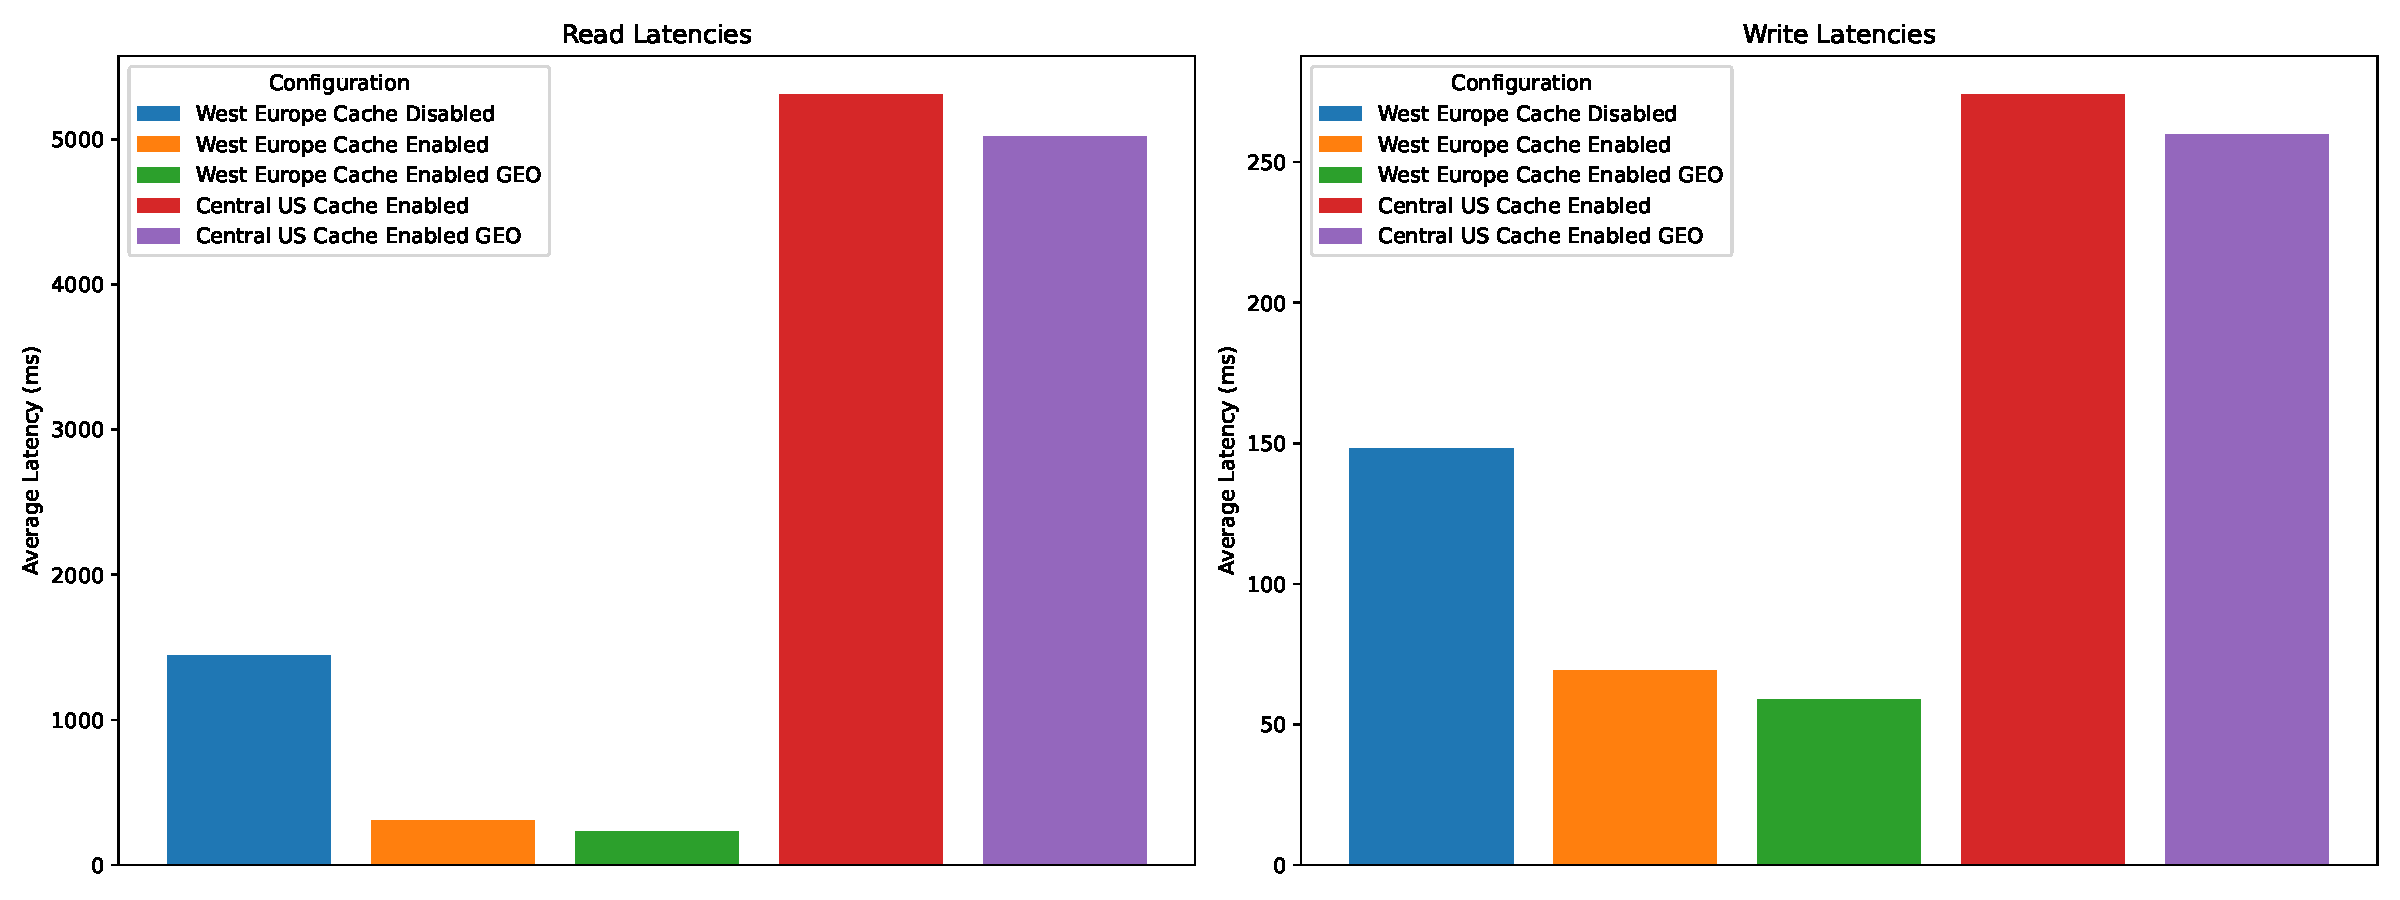
\includegraphics[width=\textwidth]{latencies.pdf}
    \caption{Average latency in milliseconds of read and write operations to different replicas, in West Europe and Central US regions, with cache enabled or disabled and using or not using geo-replication.} \label{fig:latencies}
\end{figure}

In Fig.~\ref{fig:latencies} the results of the workload tests are shown. We note that some operations require caching to function as described before (e.g., mantaining user session), and so even in the configuration with cache disabled, those operations are cached while the remaining are not.

\textbf{Caveat}: The read latencies are much greater than the write latencies because of implementations details regarding how we treat deleted users, e.g., when listing an auction's questions the app service checks sequentially each user in each question. This can be optimized with some approaches, e.g., getting the user information in bulk, denormalizing the data.

Nonetheless, we can observe that having cache enabled greatly reduces the client perceived latency, in read latency by a factor of 5 and in write of 2 in this case. This is because the app service eventually gets most pre-computed information that operations need from cache without the need of querying the database, as is the main goal of caching.

It can also be noticed that having geo-replication does not affect the perceived latency. This is because all operations have session consistency level, except for the two mentioned before, and so the West Europe replica doesn't need to make sure the Central US replica has received its replicated writes before returning to the client. 

\section{Conclusion}

In this work, we presented a backend system for an auction based service like E-Bay operating on cloud infrastruture, taking advantage of cloud computing technics to support its functionality. 

Our system in particular is able to handle concurrent bids using conditional updates, provides caching of previously computed data to speed up operations, uses multiple serverless functions to support some functionality like closing of auctions, and provides advanced search with text based queries.

Through the evaluation, we can conclude that using our system with cache is worthwhile to reduce significantly the latency perceived by clients, and geo-replication is also useful to improve fault tolerance, while causing little to no effect on operation latency. 

\end{document}
